
Electromagnetic transient (EMT) simulation focuses on resolving the instantaneous 
behaviour of electrical networks when they are subject to fast and often severe disturbances.
 Unlike RMS or phasor-domain studies, which assume that voltages and currents remain 
 approximately sinusoidal within each time step, EMT models compute these quantities directly 
 in the time domain. This makes it possible to capture the full electromagnetic response of components, 
 including switching actions, resonances, travelling waves, and short-duration dynamic interactions 
 between converters and the grid.

Modern EMT tools are based on the numerical formulation introduced by Dommel 
in the late 1960s and subsequently used in the Electromagnetic Transients Program (EMTP)~\cite{Dommel_EMTP_Theory_Book_1986}.
In this approach, each network element is represented through an equivalent conductance and a history-dependent 
current source. By assembling all contributions at every time step, the simulator solves a linear algebraic 
system of the form:


\begin{equation}
    [G]~[v(t)] = [i(t)]-[I_{\text{hist}}]
\end{equation}

where $[G]$ is the global conductance matrix of the network, $v(t)$ is the vector of node voltages, 
$i(t)$ contains the instantaneous current injections, and $i_{\text{hist}}(t)$ represents the history terms 
accumulated from previous time steps. This formulation is flexible and allows linear, nonlinear, 
and power-electronic elements to be incorporated into the same solution process. This type of solver is called a 
Modified Nodal Analysis (MNA) solver. 

%The time-step size in EMT simulations is typically in the order of microseconds to capture high-frequency events while 

EMT simulation is essential whenever the assumptions of RMS-based dynamic studies no longer hold. 
RMS models use phasors to represent voltages and currents, and they rely on the idea that the waveform remains nearly sinusoidal. 
This approximation is often sufficient for analysing electromechanical behaviour, such as rotor-angle stability, 
slow voltage dynamics, or generator control interactions, where the dominant time constants range from tens of milliseconds 
to several seconds~\cite{StabilityAndControlKundur}.

However, RMS models inherently filter out high-frequency and sub-cycle behaviour. They cannot accurately represent:
\begin{itemize}
    \item Switching transients in power-electronic converters.
    \item Transformer inrush and magnetic saturation.
    \item Lightning impulses and surge propagation.
    \item Fast protection and relay actions.
    \item Travelling waves on overhead lines and underground cables.
    \item Harmonic and resonance interactions.
    \item Instabilities driven by phase-locked loops or weak-grid conditions.
\end{itemize}

All these phenomena unfold at microsecond to millisecond time scales and require explicit time-domain resolution. 
EMT simulation is therefore the only method capable of capturing the detailed electromagnetic response of a system 
under such conditions. This has become particularly important in converter-dominated grids, where the interaction between 
fast control loops and grid dynamics may lead to oscillations or instabilities that RMS simulations cannot reveal.

In practice, EMT simulation is used to:
\begin{itemize}
    \item Analyse the internal behaviour of converter controllers,
    \item Validate protection algorithms relying on high-speed measurements,
    \item Assess resonance propagation along cables and transformers,
    \item Evaluate insulation coordination and surge propagation,
    \item Study black-start and grid-forming behaviour,
    \item Examine the detailed impact of grid faults on converter-rich systems.
\end{itemize}

Although RMS and EMT simulations aim to describe power-system behaviour, they operate at very different levels of detail. 
The main conceptual differences are summarised below:
\begin{itemize}
    \item \textit{Waveform representation:}  
    RMS models use phasors, assuming sinusoidal waveforms with slowly varying magnitude and phase.  
    EMT models compute instantaneous voltages and currents, allowing arbitrary waveform distortion.

    \item \textit{Time resolution:}  
    RMS simulations typically use time steps between 1--10~ms.  
    EMT simulations use time steps in the range of 20--50~$\mu$s, or even smaller when needed.

    \item \textit{Phenomena captured:}  
    RMS simulations focus on electromechanical dynamics and long-term voltage behaviour.  
    EMT simulations capture electromagnetic transients, converter switching, resonances, saturation, and sub–cycle interactions.

    \item \textit{Computational requirements:}  
    RMS simulations are computationally efficient and scale well to large networks.  
    EMT simulations require significantly more computation but provide the detail needed to study fast or nonlinear phenomena.
\end{itemize}

Both approaches are complementary. RMS simulation remains essential for system-wide stability and planning studies, 
while EMT simulation is indispensable for detailed transient analysis, validation of protection schemes, and the study of 
power-electronic behaviour in modern grids.

\subsection{Line Model: Bergeron's Model}

Accurate modelling of transmission lines is essential in electromagnetic transient (EMT) simulation because wave propagation, reflections, 
and attenuation determine the fast behaviour of the network during disturbances. Lumped representations such as the classical $\pi$-model 
are widely used in steady-state and RMS dynamic analysis; however, their structural assumptions make them inadequate for EMT studies. 
A $\pi$-model represents the line using a single series impedance and two shunt admittances, implicitly assuming that the line is electrically 
short relative to the wavelength of interest and that propagation effects can be neglected. 
Such a representation introduces neither the propagation delay nor the distributed nature of the line parameters, and therefore cannot 
reproduce travelling waves, reflection phenomena, refraction at line terminations, or frequency-dependent attenuation.
 Although subdividing the line into multiple cascaded $\pi$-sections improves accuracy, it also increases numerical stiffness 
 and computational cost, making it unsuitable as the foundation of an EMT solver \cite{Dommel_EMTP_Theory_Book_1986}.

For EMT simulation, the model must preserve the distributed nature of the line as described by the telegrapher's equations. 
A representation fulfilling this requirement while remaining computationally efficient is the Bergeron travelling-wave model, originally 
formulated for EMTP-type tools. The model introduces the characteristic impedance and the propagation delay directly into the nodal formulation, 
enabling a physically meaningful description of wave propagation with excellent numerical stability. This makes Bergeron's method particularly 
appropriate for the development of foundational EMT solvers.

\subsubsection{From Telegrapher's Equations to the Bergeron's line Model}

For a lossless transmission line, the distributed parameters reduce to an inductance per unit length $L'$ and a capacitance per unit length $C'$.
Under this assumption, the telegrapher's equations take the form:

\begin{equation}
    \frac{\partial v(x,t)}{\partial x} = -L' \frac{\partial i(x,t)}{\partial t},
\end{equation}
\begin{equation}
    \frac{\partial i(x,t)}{\partial x} = -C' \frac{\partial v(x,t)}{\partial t}.
\end{equation}

Differentiating each equation with respect to $x$ and $t$ and substituting leads to two wave equations:

\begin{equation}
    \frac{\partial^2 v(x,t)}{\partial x^2} = L' C' \frac{\partial^2 v(x,t)}{\partial t^2},
\end{equation}
\begin{equation}
    \frac{\partial^2 i(x,t)}{\partial x^2} = L' C' \frac{\partial^2 i(x,t)}{\partial t^2}.
\end{equation}

The general solution of these equations is a superposition of forward- and backward-travelling waves,

\begin{equation}
    v(x,t) = v^{+}(t - x/v) + v^{-}(t + x/v),
\end{equation}
\begin{equation}
    i(x,t) = \frac{1}{Z_c} v^{+}(t - x/v) - \frac{1}{Z_c} v^{-}(t + x/v),
\end{equation}

where the characteristic impedance and wave velocity are
\begin{equation}
    Z_c = \sqrt{\frac{L'}{C'}}, \qquad v = \frac{1}{\sqrt{L' C'}}.
\end{equation}

At the sending terminal ($x=0$) and receiving terminal ($x=\ell$), these expressions become:

\begin{equation}
    v_f(t) = v^{+}(t) + v^{-}(t),
\end{equation}
\begin{equation}
    i_f(t) = \frac{1}{Z_c}\big( v^{+}(t) - v^{-}(t) \big),
\end{equation}
\begin{equation}
    v_t(t) = v^{+}(t - \tau) + v^{-}(t + \tau),
\end{equation}
\begin{equation}
    i_t(t) = \frac{1}{Z_c}\big( v^{+}(t - \tau) - v^{-}(t + \tau) \big),
\end{equation}
where $\tau = \ell / v$ is the propagation delay.

Solving these relationships for $v^{+}$ and $v^{-}$ and eliminating them yields the Norton-type expressions used in the Bergeron's model. 
The current at each terminal can be written as the sum of an instantaneous contribution through the characteristic impedance and a 
history-dependent term:
\begin{equation}
    i_{\text{f,t}}(t) = \frac{1}{Z_c} v_\text{f}(t) + I_{\text{hist,f}}(t - \tau),
\end{equation}
\begin{equation}
    i_{\text{t,f}}(t) = \frac{1}{Z_c} v_\text{t}(t) + I_{\text{hist,t}}(t - \tau),
\end{equation}
with history currents
\begin{equation}
    I_{\text{hist,f}}(t-\tau) = -\frac{1}{Z_c} v_\text{t}(t-\tau) - i_{\text{t,f}}(t-\tau),
\end{equation}
\begin{equation}
    I_{\text{hist,t}}(t-\tau) = -\frac{1}{Z_c} v_\text{f}(t-\tau) - i_{\text{f,t}}(t-\tau).
\end{equation}

This formulation expresses each terminal of the line as a Norton equivalent consisting of a conductance $1/Z_c$ in parallel with a 
current source dependent on delayed voltages and currents. As a result, the model integrates naturally into the nodal-analysis framework of
EMT solvers and preserves the essential physics of wave propagation. 

Figure \ref{fig:bergeron_lossless} illustrates the Bergeron's lossless line model, highlighting the characteristic impedance and history-current sources.

\begin{figure}[H]
  \centering
  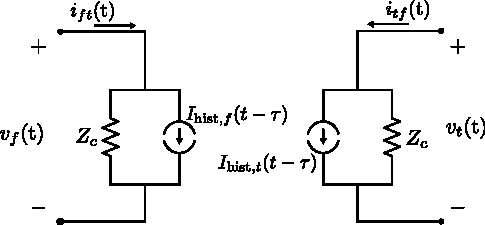
\includegraphics[width=0.6\linewidth]{inkscape_svg/bergeron_lossless.pdf}
  \caption{Bergeron's lossless line model.}
  \label{fig:bergeron_lossless}
\end{figure}

\subsubsection{Bergeron's line Model with Lumped Resistances}

Real transmission lines exhibit losses; therefore, the model must incorporate attenuation. A standard EMT approximation 
introduces the total series resistance $R$ by splitting the line into two halves and representing each half with its own 
Bergeron equivalent.Each halve has $R/4$ resistances added to each terminal, effectively distributing the losses along 
the line. Figure~\ref{fig:bergeron_losses} shows this configuration.

\begin{figure}[H]
  \centering
  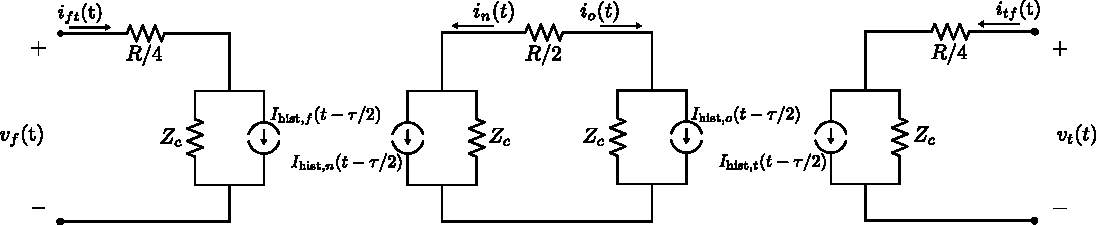
\includegraphics[width=1\linewidth]{inkscape_svg/bergeron_with_losses_full.pdf}
  \caption{Bergeron's line model with lumped resistance.}
  \label{fig:bergeron_losses}
\end{figure}

Splitting the resistance modifies the apparent characteristic impedance of each half-line. The equivalent becomes
\begin{equation}
    Z = Z_c + \frac{R}{4},
\end{equation}
because each resistor of value $R/2$ is divided in two and attached symmetrically to each end. This adjustment introduces 
attenuation in the travelling wave components. The attenuation coefficient is defined as
\begin{equation}
    H = \frac{Z_c - R/4}{Z_c + R/4},
\end{equation}
and governs the damping of each travelling wave as it propagates through the resistive sections.

The half-line equivalent, shown in Fig.~\ref{fig:bergeron_losses_half}, leads to a history current of the form:
\begin{figure}[H]
  \centering
  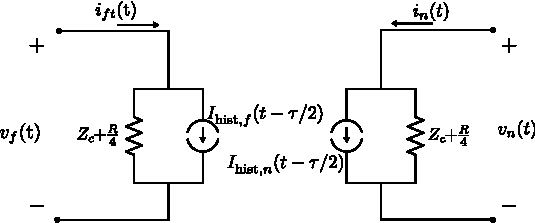
\includegraphics[width=0.6\linewidth]{inkscape_svg/bergeron_half_line_losses.pdf}
  \caption{Half Bergeron line model with lumped resistance.}
  \label{fig:bergeron_losses_half}
\end{figure}

\begin{equation}
 I_{\text{hist,m}}(t-\tau/2)
    = -\frac{1}{Z_c + R/4} v_\text{m}(t-\tau/2)
      - H \, i_\text{m}(t-\tau/2).
\end{equation}

This expression already reflects both the propagation delay and the attenuation due to the series resistance.

To recover a two-terminal equivalent, the contributions of the two half-lines are combined, producing the structure in 
Fig.~ \ref{fig:bergeron_losses_equiv}. The resulting history current at the sending terminal is a weighted combination of 
delayed voltages and currents at both ends:
\begin{figure}[H]
  \centering
  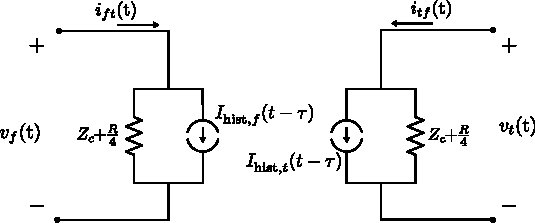
\includegraphics[width=0.6\linewidth]{inkscape_svg/bergeron_losses_equivalent.pdf}
  \caption{Bergeron's line model with lumped resistance two-nodes equivalent.}
  \label{fig:bergeron_losses_equiv}
\end{figure}

\begin{equation}
\begin{aligned}
    I_{\mathrm{hist},f}(t-\tau)
    &= \left(\frac{1+H}{2}\right)
       \left(-\frac{1}{Z}v_t(t-\tau)-i_{t,f}(t-\tau)\right) \\
    &\quad + \left(\frac{1-H}{2}\right)
       \left(-\frac{1}{Z}v_f(t-\tau)-i_{f,t}(t-\tau)\right),
\end{aligned}
\end{equation}
and by symmetry,
\begin{equation}
\begin{aligned}
    I_{\mathrm{hist},t}(t-\tau)
    &= \left(\frac{1+H}{2}\right)
       \left(-\frac{1}{Z}v_f(t-\tau)-i_{f,t}(t-\tau)\right) \\
    &\quad + \left(\frac{1-H}{2}\right)
       \left(-\frac{1}{Z}v_t(t-\tau)-i_{t,f}(t-\tau)\right).
\end{aligned}
\end{equation}

This formulation retains the travelling wave nature of the line while providing a realistic approximation of 
attenuation and energy dissipation. It remains numerically stable and computationally efficient, making it well-suited for 
foundational EMT solver development. In later stages, this representation may be replaced by a frequency-dependent line model, 
which more accurately captures dispersion and broadband attenuation effects.

\subsubsection{Three-Phase and Multiconductor Line Implementation}

The travelling-wave formulation used for single-phase lines extends naturally to systems with several conductors. 
Electromagnetic transient (EMT) simulation requires explicit representation of each conductor, since fast disturbances propagate through 
coupled electromagnetic modes determined by mutual inductances and capacitances. For this reason, the implementation adopts a general 
multiconductor framework capable of modelling an arbitrary number of phases, including one-phase, two-phase, three-phase, and 
 with or without neutral configurations. This flexibility allows accurate treatment of networks where conductor geometry or availability 
 changes across sections.

The formulation begins with the computation of the distributed impedance and admittance matrices per unit length, denoted by $\mathbf{Z}'$ and 
$\mathbf{Y}'$. These matrices are derived from Carson's formulas, which incorporate both self and mutual coupling among conductors and 
remain the established foundation for overhead line parameter calculation~\cite{carson1926}. The matrices are expressed as
\begin{equation}
    \mathbf{Z}' = \mathbf{R}' + j \omega \mathbf{L}',
\end{equation}
\begin{equation}
    \mathbf{Y}' = \mathbf{G}' + j \omega \mathbf{C}'.
\end{equation}

For a Bergeron-type representation, the frequency-independent terms are extracted from $\mathbf{L}'$ and $\mathbf{C}'$. The multiconductor 
characteristic impedance and the associated conductance matrix are defined by
\begin{equation}
    \mathbf{Z}_c = \sqrt{ \mathbf{L}' \mathbf{C}' },
\end{equation}
\begin{equation}
    \mathbf{G}_c = \mathbf{Z}_c^{-1}.
\end{equation}
These expressions generalise the scalar characteristic impedance and Norton equivalent of the single-phase Bergeron's line model to the 
multiconductor case.

To incorporate attenuation effects, the distributed resistance matrix $\mathbf{R}'$ is included following the same principle as the 
single-phase lossy Bergeron model. The equivalent impedance matrix becomes
\begin{equation}
    \mathbf{Z} = \mathbf{Z}_c + \frac{1}{4}\mathbf{R}',
\end{equation}
and the attenuation matrix is defined as
\begin{equation}
    \mathbf{H} = \left( \mathbf{Z}_c - \tfrac{1}{4}\mathbf{R}' \right)
                 \left( \mathbf{Z}_c + \tfrac{1}{4}\mathbf{R}' \right)^{-1}.
\end{equation}
These matrices describe how electromagnetic waves attenuate and interact across conductors while travelling along the line.

Although $\mathbf{Z}_c$, $\mathbf{G}_c$, and $\mathbf{H}$ are treated as matrices, the propagation delay is implemented as a 
scalar quantity. This choice follows standard EMT practice: Carson's derivations produce a physically meaningful self-propagation 
velocity based on the diagonal terms of the inductance and capacitance matrices. The wave velocity is therefore computed as
\begin{equation}
    v = \frac{1}{\sqrt{L'_{\mathrm{self}} C'_{\mathrm{self}}}},
\end{equation}
and the corresponding propagation time is
\begin{equation}
    \tau = \frac{\ell}{v}.
\end{equation}
Using a single propagation delay for all conductors avoids the need for modal decomposition while maintaining adequate accuracy in 
EMT applications, particularly for transposed lines or configurations where the difference in modal velocities is small.

With this structure, each terminal of a multiconductor line contributes a Norton-type equivalent current defined by
\begin{equation}
    \mathbf{i}_f(t) = \mathbf{G}_c \, \mathbf{v}_f(t) + \mathbf{I}_{\mathrm{hist},f}(t-\tau),
\end{equation}
\begin{equation}
    \mathbf{i}_t(t) = \mathbf{G}_c \, \mathbf{v}_t(t) + \mathbf{I}_{\mathrm{hist},t}(t-\tau).
\end{equation}
The history currents are vector quantities that incorporate delayed voltages and currents from all conductors, weighted 
by the matrices $\mathbf{H}$ and $\mathbf{Z}$:
\begin{equation}
    \mathbf{I}_{\mathrm{hist},f}(t-\tau)
        = -\mathbf{Z}^{-1}\mathbf{v}_t(t-\tau)
          -\mathbf{i}_{t,f}(t-\tau),
\end{equation}
\begin{equation}
    \mathbf{I}_{\mathrm{hist},t}(t-\tau)
        = -\mathbf{Z}^{-1}\mathbf{v}_f(t-\tau)
          -\mathbf{i}_{f,t}(t-\tau).
\end{equation}

This multiconductor travelling wave representation preserves conductor coupling without requiring modal transformations 
and integrates efficiently into the global nodal formulation. It also provides a consistent basis for future upgrades to frequency-dependent 
line models, where the same matrix structure is retained while the impedance and admittance matrices become functions of frequency.



\begin{comment}
idea de com funcionar:

- tot numèric. per cada element es crea numèricament la seva pròpia G i Itotal=Isource-Ihist i després s'uneix
tot a la G i Itotal gran del sistema. 

- es fa distinció entre elements actius(generador, etc) i passius (línies, trafos...)

- Els elements actius tindran les seves equacions internes definides simbòlicament i es podran resoldre a cada timestep.
aquests tindran la tensió com a input i les iabc com a output. També d'aquest model s'ha de poder arribar al Norton equivalent:
Req i isource eq tenint en compte que les equacions internes poden ser molt diferents entre elles.

- El sistema de simulació EMT no té per a res el mateix format que RMS i no seguirà el format de blocs de RMS.

- G només canvia si hi ha events, en canvi Itotal canvia a cada pas de temps.

- S'inicialitza el sistema a 0 (s'engega tot) i quan ja està a steady state es conta tau i d'allà es pot començar a contar t=0 en endavant.

- els paràmetres/constants de cada element s'han de poder entrar com al powerflow o rms (pi-model enlloc de distributed) i internament

el sistema troba les variables correctes


- G es factoritza 1 cop i quan hi ha event i canvia es torna a factoritzar

\end{comment}
\subsection{Three-phase synchronous generator}

The synchronous generator is represented in the EMT solver as a Norton-equivalent current source in parallel with an 
admittance matrix, connected to the three-phase network at the machine terminals. At each time step, the machine model 
receives the terminal voltages, updates its internal electrical and mechanical states, and returns an equivalent current 
injection and conductance to be inserted into the modified nodal analysis (MNA) system. Figure~\ref{fig:generator_model_emt}
 illustrates the EMT-type synchronous machine model adopted in this work.

\begin{figure}[H]
  \centering
  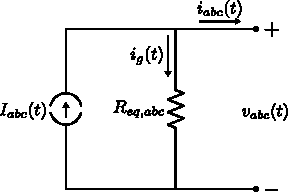
\includegraphics[width=0.45\linewidth]{inkscape_svg/generator_emt_model.pdf}
  \caption{Generator EMT-type machine model. }
  \label{fig:generator_model_emt}
\end{figure}

Where:
\begin{itemize}
    \item $v_{\text{abc}}$,  are the phase-to-neutral stator voltages,
    \item $i_{\text{abc}}$ are the phase currents injected to the network,
    \item $I_{\text{abc}}$ is the Norton-equivalent current injection from the machine to the network,
    \item $R_{\text{eq,abc}}$ is the generator Norton-equivalent impedance matrix:
    \begin{equation}
        [R_{\text{eq,abc}}] =
        \begin{bmatrix}
            R_{\text{eq,a}} & 0         & 0         \\
            0         & R_{\text{eq,b}} & 0         \\
            0         & 0         & R_{\text{eq,c}}
        \end{bmatrix},
    \end{equation}
    Which can be computed from:
    \begin{equation}
        [R_{\text{eq,dq0}}] =\begin{bmatrix}
            \frac{2~L_\text{d}''}{h} & 0         & 0         \\
            0         & \frac{2~L_\text{q}''}{h} & 0         \\
            0         & 0         & \frac{2~L_\text{0}}{h}
        \end{bmatrix},
    \end{equation}

    with  $L_\text{d}''$, $L_\text{q}''$ being the subtransient inductances in d and q axis respectively, $L_0$ the zero-axis inductance and h the simulation timestep.
    $R_{\text{eq,dq0}}$ is transformed to $R_{\text{eq,abc}}$ using the Park transformation.
    \item $i_\text{g}$ is the history current component computed from the previous state voltages.
    \begin{equation}
        i_\text{g} = \frac{1}{R_{\text{eq,abc}}}~v_{\text{abc}}(t-h)
    \end{equation}
\end{itemize}


The following assumptions are adopted for an ideal synchronous machine:
\begin{itemize}
    \item The resistance in each winding is constant.
    \item The permeance of each portion of the magnetic circuit is constant (corrections for saturation effects are introduced at a later stage).
    \item The armature windings are symmetrical with respect to each other.
    \item The electric and magnetic circuits of the field structure are symmetrical about the direct ($d$) and quadrature ($q$) axes.
    \item The self inductance of each winding on the field structure (field $f'$ and any additional rotor windings) is constant.
    \item Hysteresis effects are negligible.
    \item Eddy-current effects are negligible or, in the case of cylindrical-rotor machines, are represented by appropriate equivalent rotor windings.
\end{itemize}

For the general EMT machine model, the following additional assumptions are adopted:
\begin{itemize}
    \item Saliency effects are not neglected, i.e.\ $X_\text{d} \neq X_\text{q}$.
    \item Saturation effects are neglected in the initial model.
    \item Damper winding effects are neglected in the present implementation.
    \item The machine is represented as an equivalent two-pole machine. If the physical machine has $p$ poles, the actual angular frequency and torque are recovered as
    \begin{equation}
        \omega_{\text{actual}} = \frac{\omega_{\text{2-pole}}}{p/2},
    \end{equation}
    \begin{equation}
        T_{\text{actual}} = \frac{p}{2} \, T_{\text{2-pole}}.
    \end{equation}
    \item The quadrature axis lags the direct axis by $90^{\circ}$ electrical.
\end{itemize}

% ---------------------------------------------------
\subsubsection{Electrical part}

The electrical behaviour of the three-phase stator is described by the voltage-flux linkage equations in phase variables:
\begin{equation}
\begin{pmatrix}
v_\text{a} - i_\text{a} R_\text{a} \\
v_\text{b} - i_\text{b} R_\text{a} \\
v_\text{c} - i_\text{c} R_\text{a}
\end{pmatrix}
=
\frac{d}{dt}
\begin{pmatrix}
\psi_\text{a} \\
\psi_\text{b} \\
\psi_\text{c}
\end{pmatrix},
\end{equation}
where $v_\text{a}$, $v_\text{b}$, $v_\text{c}$ are phase-to-neutral stator voltages, $i_\text{a}$, $i_\text{b}$, $i_\text{c}$ are stator currents, $R_\text{a}$ is the stator resistance (assumed equal in all phases), and $\psi_\text{a}$, $\psi_\text{b}$, $\psi_\text{c}$ are the corresponding flux linkages. The field winding (referred to the stator) satisfies
\begin{equation}
    v_{\text{f}'} - i_{\text{f}'} R_{\text{f}'} = \frac{d \psi_{\text{f}'}}{dt},
\end{equation}
where $v_{\text{f}'}$ is the field voltage, $i_{\text{f}'}$ is the field current, $R_{\text{f}'}$ is the field resistance and $\psi_{\text{f}'}$ is the field flux linkage.

For the EMT formulation, it is convenient to express the stator quantities in the rotating $dq$ reference frame using the Park transformation. The transformation from $\text{abc}$ to $\text{dq0}$ variables is
\begin{equation}
    [T(\theta)] =
    \frac{2}{3}
    \begin{bmatrix}
        \cos(\theta)                 & \cos\!\left(\theta - \tfrac{2\pi}{3}\right) & \cos\!\left(\theta + \tfrac{2\pi}{3}\right) \\[6pt]
        \sin(\theta)                 & \sin\!\left(\theta - \tfrac{2\pi}{3}\right) & \sin\!\left(\theta + \tfrac{2\pi}{3}\right) \\[6pt]
        \tfrac{1}{2}                 & \tfrac{1}{2}                                 & \tfrac{1}{2}
    \end{bmatrix},
\end{equation}
and the inverse transformation is
\begin{equation}
    [T(\theta)]^{-1} =
    \begin{bmatrix}
        \cos(\theta)                 & \sin(\theta)                 & 1 \\[6pt]
        \cos\!\left(\theta - \tfrac{2\pi}{3}\right) & \sin\!\left(\theta - \tfrac{2\pi}{3}\right) & 1 \\[6pt]
        \cos\!\left(\theta + \tfrac{2\pi}{3}\right) & \sin\!\left(\theta + \tfrac{2\pi}{3}\right) & 1
    \end{bmatrix}.
\end{equation}

In the $\text{dq0}$ reference frame and for the simplified model considered (one field winding, no explicit damper windings), the stator $d$- and $q$-axis voltage equations take the form
\begin{equation}
    v_\text{d} = R_\text{a} i_\text{d} + \frac{d} \psi_\text{d}{dt} - \omega \psi_\text{q},
\end{equation}
\begin{equation}
    v_\text{q} = R_\text{a} i_\text{q} + \frac{d} \psi_\text{q}{dt} + \omega \psi_\text{d},
\end{equation}
\begin{equation}
    v_\text{0} = R_\text{0} i_\text{0} 
\end{equation}
and the field equation becomes
\begin{equation}
    v_{\text{f}'} = R_{\text{f}'} i_{\text{f}'} + \frac{d \psi_{\text{f}'}}{dt}.
\end{equation}

Flux linkages are expressed in terms of currents through the $d$- and $q$-axis inductances. For the $d$-axis, including stator leakage inductance $L_\text{a}$, magnetising inductance $L_{\text{md}}$ and field inductance (referred to stator) $L_\text{a}$ for the $\text{f}'$ winding, the relations are
\begin{equation}
\begin{pmatrix}
\psi_\text{d} \\
\psi_{\text{f}'}
\end{pmatrix}
=
\begin{bmatrix}
L_{\text{md}} + L_\text{a} & L_{\text{md}} \\
L_{\text{md}}       & L_{\text{md}} + L_\text{a}
\end{bmatrix}
\begin{pmatrix}
i_\text{d} \\
i_{\text{f}'}
\end{pmatrix},
\end{equation}
whereas for the $q$-axis (with magnetising inductance $L_{\text{mq}}$ and stator leakage $L_\text{a}$),
\begin{equation}
    \psi_\text{q} = (L_{\text{mq}} + L_\text{a}) \, i_\text{q}.
\end{equation}

Figure~\ref{fig:generator_dq_models} shows the equivalent $d$- and $q$-axis circuit representations corresponding to these equations.


\begin{figure}
\centering
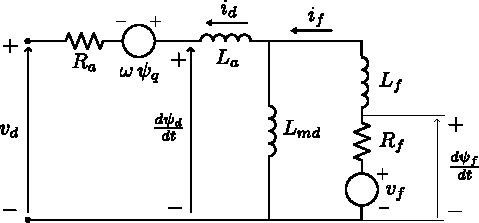
\includegraphics[width=0.8\linewidth]{inkscape_svg/generator_daxis_model.pdf}
\caption{Generator $d$-axis equivalent model.}
\label{fig:generator_daxis_model}
\end{figure}

\begin{figure}
\centering
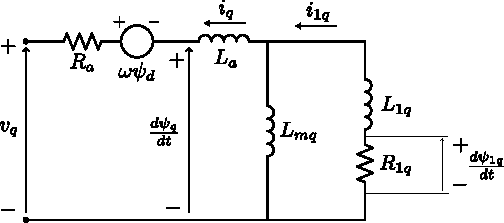
\includegraphics[width=0.77\linewidth]{inkscape_svg/generator_qaxis_model.pdf}
\caption{Generator $q$-axis equivalent model.}
\label{fig:generator_qaxis_model}
\end{figure}


The electromagnetic torque is obtained from the $dq$ quantities as
\begin{equation}
    T_\text{e} = \frac{3}{2} \left( \psi_\text{d} i_\text{q} - \psi_\text{q} i_\text{d} \right),
\end{equation}
which is consistent with the adopted sign convention. This expression is used both in the mechanical equations and in the symbolic implementation of the model.

% ---------------------------------------------------
\subsubsection{Mechanical part}

The mechanical dynamics of the rotor are described by a two-state system in rotor angle $\theta$ and speed $\omega$. 
In continuous time, the mechanical equations can be written as
\begin{equation}
\frac{d}{dt}
\begin{pmatrix}
\theta \\[4pt]
\omega
\end{pmatrix}
=
\begin{pmatrix}
0 & 1 \\[4pt]
0 & -\dfrac{D}{J}
\end{pmatrix}
\begin{pmatrix}
\theta \\[4pt]
\omega - \omega_{ref}
\end{pmatrix}
+
\begin{pmatrix}
0 \\[4pt]
\dfrac{T_{m} - T_{e}}{J}
\end{pmatrix},
\end{equation}
where $J$ is the rotor inertia, $D$ is the damping coefficient, $T_m$ is the mechanical torque and $T_e$ is 
the electromagnetic torque. In per-unit form, and using the inertia constant $H$ and base speed $\omega_b$, 
the equations are commonly written as
\begin{equation}
    \frac{d \theta}{dt}(t) = \omega_\text{b} \, (\omega(t) - \omega_{\text{ref}}),
\end{equation}
\begin{equation}
    \frac{d \omega}{dt}(t)
    = \frac{\Gamma_\text{m}(t) - \Gamma_\text{e}(t) - D (\omega(t) - \omega_{\text{ref}})}{2 H},
\end{equation}
with
\begin{equation}
    \Gamma_\text{m}(t) = \frac{P(t)}{\omega},
\end{equation}
\begin{equation}
    \Gamma_\text{e}(t) = \frac{3}{2} \left( i_\text{d}(t) \psi_\text{q}(t) - i_\text{q}(t) \psi_\text{d}(t) \right),
\end{equation}
where $P(t)$ is the mechanical power input, and $\Gamma_\text{m}$, $\Gamma_\text{e}$ denote mechanical and electromagnetic torque in per-unit.

% ---------------------------------------------------
\subsubsection{Parameters determination}

The EMT model requires inductances and resistances in the $dq$ reference frame, while manufacturers typically 
provide parameters in the form of synchronous, transient and subtransient reactances and time constants. The known quantities are
\begin{itemize}
    \item $R_\text{a}$: armature resistance (also called stator resistance),
    \item $X_\text{l}$: armature leakage reactance,
    \item $X_\text{0}$: zero-sequence reactance,
    \item $R_\text{0}$: zero-sequence resistance,
    \item $X_\text{d}$, $X_\text{q}$: synchronous reactances,
    \item $X_\text{d}'$, $X_\text{q}'$: transient reactances,
    \item $X_\text{d}''$, $X_\text{q}''$: subtransient reactances,
    \item $T_\text{d}'$, $T_\text{q}'$: transient short-circuit time constants,
    \item $T_\text{d}''$, $T_\text{q}''$: subtransient short-circuit time constants.
\end{itemize}

From these quantities, the required inductances and rotor parameters are obtained by standard relations. For the $d$-axis,
\begin{equation}
    L_\text{d} = \frac{X_\text{d}}{\omega_\text{b}}, \qquad
    L_\text{d}' = \frac{X_\text{d}'}{\omega_\text{b}}, \qquad
    L_\text{d}'' = \frac{X_\text{d}''}{\omega_\text{b}},
\end{equation}
and similarly for the $q$-axis,
\begin{equation}
    L_\text{q} = \frac{X_\text{q}}{\omega_\text{b}}, \qquad
    L_\text{q}' = \frac{X_\text{q}'}{\omega_\text{b}}, \qquad
    L_\text{q}'' = \frac{X_\text{q}''}{\omega_\text{b}}.
\end{equation}
The magnetising inductances and rotor inductances are derived from these effective inductances and the leakage component. For instance,
\begin{equation}
    L_{\text{md}} = L_\text{d} - L_\text{a},
\end{equation}
and the rotor branch inductances and resistances are determined from the differences between $L_\text{d}$, $L_\text{d}'$, $L_\text{d}''$ 
and the corresponding time constants. An analogous procedure is followed for the $q$-axis. These calculations provide 
$L_{\text{md}}$, $L_{\text{mq}}$, $L_\text{a}$, $L_{\text{f}'}$, and any additional rotor parameters required by the selected level of detail.

% ---------------------------------------------------
\subsubsection{Transient solution}

At each EMT time step, the synchronous machine model is advanced using the network solution from the previous
iteration and the internal electrical and mechanical states of the generator. The complete procedure is summarised below.

\begin{enumerate}
    \item \textit{Park transformation of terminal voltages.}  
    The stator terminal voltages in $abc$ coordinates at the previous time step $t-h$ are transformed to $\text{dq0}$ variables using
    \begin{equation}
        [v_{\text{dq0}}(t-h)] = [T(\theta(t-h))] \, [v_{\text{abc}}(t-h)],
    \end{equation}
    where
    \begin{equation}
    [T(\theta)] =
    \frac{2}{3}
    \begin{bmatrix}
    \cos(\theta)                & \cos(\theta - \tfrac{2\pi}{3}) & \cos(\theta + \tfrac{2\pi}{3}) \\[6pt]
    \sin(\theta)                & \sin(\theta - \tfrac{2\pi}{3}) & \sin(\theta + \tfrac{2\pi}{3}) \\[6pt]
    \tfrac{1}{2}                & \tfrac{1}{2}                   & \tfrac{1}{2}
    \end{bmatrix}.
    \end{equation}

    \item \textit{Evaluation of flux-derivative terms.}  
    Using the electrical equations in the $dq0$ frame, the derivatives of the flux linkages are computed at time $t$ based on known quantities at $t-h$:
    \begin{equation}
    \begin{aligned}
    v_\text{d} &= R_\text{a} i_\text{d} + \frac{d\psi_\text{d}}{dt} - \omega \psi_\text{q}, \\[4pt]
    v_\text{q} &= R_\text{a} i_\text{q} + \frac{d\psi_\text{q}}{dt} + \omega \psi_\text{d}, \\[4pt]
    v_\text{0} &= R_\text{a} i_\text{0} + \frac{d\psi_\text{0}}{dt}.
    \end{aligned}
    \end{equation}

    The field voltage equation remains
    \begin{equation}
    v_{\text{f}'} = R_{\text{f}'} i_{\text{f}'} + \frac{d\psi_{\text{f}'}}{dt}.
    \end{equation}

    Thus, the flux derivatives evaluated at time $t$ using information at time $t-h$ are:
    \begin{equation}
    \begin{aligned}
    \frac{d\psi_\text{d}}{dt}(t) &= v_\text{d}(t-h) - R_\text{a} i_\text{d}(t-h) - \omega(t-h)\psi_\text{q}(t-h), \\[4pt]
    \frac{d\psi_\text{q}}{dt}(t) &= v_\text{q}(t-h) - R_\text{a} i_\text{q}(t-h) + \omega(t-h)\psi_\text{d}(t-h), \\[4pt]
    \frac{d\psi_\text{0}}{dt}(t) &= v_\text{0}(t-h) - R_\text{a} i_\text{0}(t-h), \\[4pt]
    \frac{d\psi_{\text{f}'}}{dt}(t) &= v_{\text{f}'}(t-h) - R_{\text{f}'} i_{\text{f}'}(t-h).
    \end{aligned}
    \label{eq:dq0_flux_derivatives}
    \end{equation}

    \item \textit{Trapezoidal integration of flux linkages.}  
    The fluxes at the new time step $t$ are obtained by trapezoidal integration:
    \begin{equation}
        \begin{aligned}
            \psi_\text{d}(t) &= \psi_\text{d}(t-h) + h \, \frac{\tfrac{d \psi_\text{d}(t)}{d t} + \tfrac{d \psi_\text{d}(t-h)}{d t}}{2}, \\
            \psi_{\text{f}'}(t) &= \psi_{\text{f}'}(t-h) + h \, \frac{\tfrac{d \psi_{\text{f}'}(t)}{d t} + \tfrac{d \psi_{\text{f}'}(t-h)}{d t}}{2}, \\
            \psi_\text{q}(t) &= \psi_\text{q}(t-h) + h \, \frac{\tfrac{d \psi_\text{q}(t)}{d t} + \tfrac{d \psi_\text{q}(t-h)}{d t}}{2}. \\
            \psi_\text{0}(t) &= \psi_\text{0}(t-h) + h \, \frac{\tfrac{d \psi_\text{0}(t)}{d t} + \tfrac{d \psi_\text{0}(t-h)}{d t}}{2}.
        \end{aligned}
    \end{equation}

    \item \textit{Computation of $\text{dq0}$ currents.}  
    Once the new flux linkages are known, the $\text{dq0}$-axis currents are obtained from
    \begin{equation}
        \begin{pmatrix}
        i_\text{d}(t) \\
        i_{\text{f}'}(t) 
        \end{pmatrix}
        =
        [L_\text{d}]^{-1}
        \begin{pmatrix}
        \psi_\text{d}(t) \\
        \psi_{\text{f}'}(t)
        \end{pmatrix},
    \end{equation}
    where
    \begin{equation}
        [L_\text{d}] =
        \begin{bmatrix}
        L_{\text{md}} + L_\text{a} & L_{\text{md}} \\[6pt]
        L_{\text{md}}       & L_{\text{md}} + L_\text{a}
        \end{bmatrix},
    \end{equation}
    for the $q$-axis current is
    \begin{equation}
        i_\text{q}(t) = \frac{\psi_\text{q}(t)}{L_{\text{mq}} + L_\text{a}}.
    \end{equation}
    and for the 0-axis current:
    \begin{equation}
        i_\text{0}(t) = \frac{\psi_\text{0}(t)}{L0}.
    \end{equation}

    \item \textit{Update of mechanical states.}  
    With $i_\text{d}(t)$, $i_\text{q}(t)$, $\psi_\text{d}(t)$, $\psi_\text{q}(t)$ available, the electromagnetic torque $\Gamma_\text{e}(t)$ is computed as
    \begin{equation}
        \Gamma_\text{e}(t) = -\frac{3}{2} \left( i_\text{d}(t) \psi_\text{q}(t) - i_\text{q}(t) \psi_\text{d}(t) \right).
    \end{equation}
    The mechanical equations are then integrated (e.g.\ by trapezoidal rule) to obtain the updated $\omega(t)$ and $\theta(t)$, using
    \begin{equation}
        \frac{d \theta}{dt}(t) = \omega_\text{b} (\omega(t)),
    \end{equation}
    \begin{equation}
        \frac{d \omega}{dt}(t) = \frac{\Gamma_\text{m}(t) - \Gamma_\text{e}(t) - D(\omega(t) - \omega_{\text{ref}})}{2 H}.
    \end{equation}

    \item \textit{Equivalent Norton quantities in $\text{dq0}$.}  
    The Norton-equivalent current injection in the $\text{dq0}$ frame is obtained from an equivalent conductance matrix $[G_{\text{eq,dq}}]$ as
    \begin{equation}
        [I_{\text{g,dq0}}(t)] = [G_{\text{eq,dq0}}] \, [v_{\text{dq0}}(t-h)]
    \end{equation}
    The specific form of $[G_{\text{eq,dq0}}]$ follows from the trapezoidal discretisation of the $\text{dq0}$-axis circuit equations.

    \item \textit{Transformation back to $\text{abc}$ and MNA insertion.}  
    The $\text{dq0}$ currents and Norton current injection are transformed back to phase coordinates using
    \begin{equation}
        [i_{\text{abc}}(t)] = [T(\theta(t))]^{-1} [i_{\text{dq0}}(t)],
    \end{equation}
    \begin{equation}
        [i_{\text{g,abc}}(t)] = [T(\theta(t))]^{-1} [I_{\text{g,dq0}}(t)],
    \end{equation}
    and the equivalent conductance matrix in $abc$ coordinates is
    \begin{equation}
        [G_{\text{eq,abc}}(t)] = [T(\theta(t))]^{-1} [G_{\text{eq,dq0}}]  [T(\theta(t))].
    \end{equation}
    Finally, the Norton-equivalent current source to be inserted into the network is
    \begin{equation}
        [I_{\text{g,abc}}(t)] = [i_{\text{abc}}(t)] + [G_{\text{eq,abc}}(t)] [v_{\text{abc}}(t-h)].
    \end{equation}
    These contributions are added to the global MNA system to obtain the network solution at the next time step.
\end{enumerate}

Figure~ \ref{fig:machine_net_sol} shows the overall interaction between the machine model and the network solution at each time step.

\begin{figure}[H]
\centering
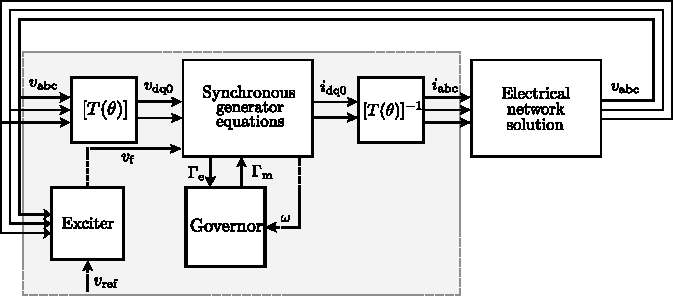
\includegraphics[width=1\linewidth]{inkscape_svg/machine_network_solution.pdf}
\caption{Generator EMT-type machine model and network solution process at each time step.}
\label{fig:machine_net_sol}
\end{figure}

In the EMTDC program, synchronous machines are represented in the network by means of current injections 
formulated through the system admittance matrix. As in any current-injection-based interface, the injected currents are computed 
using terminal voltages from previous time-steps. Consequently, an abrupt change in the terminal voltage does not influence the injected 
current until the following time step, which effectively causes the machine to behave as an open circuit during that interval. 
This numerical delay may produce artificial voltage spikes at the machine terminals. When several machines are connected within the same 
subsystem, the cumulative effect of these spikes can compromise numerical stability. To mitigate this issue, the machine model is augmented 
with an interfacing resistor, which introduces a direct voltage-current coupling and significantly improves the robustness of the numerical 
solution \cite{WatsonArrillagaEMT2019}. 

The value of this resistor should be chosen carefully to balance numerical stability and physical accuracy. Each comercial EMT software uses its own criteria
being R between 10 and 20 times the base impedance a common choice. In VeraGrid, the interfacing resistor is set to 20 times the base impedance of the machine.
The equivalent circuit of the generator model including the interfacing resistor is shown in Figure~\ref{fig:generator_emt_model_resistor}.

\begin{figure}[H]
\centering
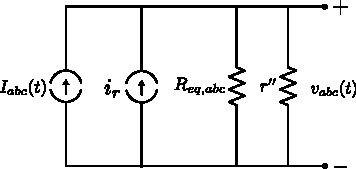
\includegraphics[width=0.45\linewidth]{inkscape_svg/generator_emt_model_interfacing_resistor.pdf}
\caption{Generator EMT-type machine model including the interfacing resistor.}
\label{fig:generator_emt_model_resistor}
\end{figure}



% ---------------------------------------------------
\subsubsection{VeraGrid implementation}

The generator EMT-type machine model is implemented in VeraGrid using symbolic blocks. Since the derivatives of the 
state variables are required at each time step, the state variables are explicitly declared as differential variables 
in the symbolic representation. The state variables are $\psi_\text{d}$, $\psi_{\text{f}'}$, $\psi_\text{q}$, $\psi_\text{0}$, $\theta$ and $\omega$, 
with differential equations:
\begin{equation}
\begin{cases}
\displaystyle \frac{d \psi_\text{d}}{dt} = v_\text{d} - i_\text{d} R_\text{a} - \omega \psi_\text{q}, \\[6pt]
\displaystyle \frac{d \psi_{\text{f}'}}{dt} = v_{\text{f}'} - R_{\text{f}'} i_{\text{f}'}, \\[6pt]
\displaystyle \frac{d \psi_\text{q}}{dt} = v_\text{q} - R_\text{a} i_\text{q} + \omega \psi_\text{d}, \\[6pt]
\displaystyle \frac{d \psi_\text{0}}{dt} = v_\text{0} - R_\text{a} i_\text{0} \\[6pt]
\displaystyle \frac{d \theta}{dt} = \omega_\text{b}~\omega, \\[6pt]
\displaystyle \frac{d \omega}{dt} = \frac{\Gamma_\text{m} - \Gamma_\text{e} - D(\omega - \omega_{\text{ref}})}{2 H}
\end{cases}
\label{eq:diff_eq_gen}
\end{equation}

The corresponding algebraic equations include the electromagnetic torque, flux-current relations and Park transformations:
\begin{equation}
\begin{cases}
\Gamma_\text{e} = -\dfrac{3}{2} (i_\text{d} \psi_\text{q} - i_\text{q} \psi_\text{d}), \\[6pt]
\psi_\text{d} = (L_{\text{md}} + L_\text{a}) i_\text{d} + L_{\text{md}} i_{\text{f}'}, \\[6pt]
\psi_{\text{f}'} = L_{\text{md}} i_\text{d} + (L_{\text{md}} + L_\text{f'}) i_{\text{f}'}, \\[6pt]
\psi_\text{q} = (L_{\text{mq}} + L_\text{a}) i_\text{q}, \\[6pt]
\psi_\text{0} = (L_\text{0}) i_\text{0}, \\[6pt]
P_\text{e} = v_\text{a} i_\text{a} + v_\text{b} i_\text{b} + v_\text{c} i_\text{c}, \\[6pt]
Q_\text{e} - (1 / \sqrt(3))~ ((v_\text{a} - v_\text{b})~ i_\text{c} + (v_\text{b} - v_\text{c})~ i_\text{a} + (v_\text{c} - v_\text{a})~ i_\text{b}),
i_\text{a} = \cos(\theta) i_\text{d} + \sin(\theta) i_\text{q} + i_\text{0}, \\[6pt]
i_\text{b} = \cos(\theta - 2\pi/3) i_\text{d} + \sin(\theta - 2\pi/3) i_\text{q} + i_\text{0}, \\[6pt]
i_\text{c} = \cos(\theta + 2\pi/3) i_\text{d} + \sin(\theta + 2\pi/3) i_\text{q} + i_\text{0}, \\[6pt]
v_\text{d} = \cos(\theta) v_\text{a} + \cos(\theta - 2\pi/3) v_\text{b} + \cos(\theta + 2\pi/3) v_\text{c}, \\[6pt]
v_\text{q} = \sin(\theta) v_\text{a} + \sin(\theta - 2\pi/3) v_\text{b} + \sin(\theta + 2\pi/3) v_\text{c}, \\[6pt]
v_\text{0} = 0,5 v_\text{a} + 0,5 v_\text{b} + 0,5 v_\text{c} \\[6pt]
\end{cases}
\label{eq:alg_eq_gen}
\end{equation}

The variables $v_\text{a}$, $v_\text{b}$ and $v_\text{c}$ are taken from the network solution at the bus where the generator is connected. 
The field voltage $v_{\text{f}'}$ must be provided by the exciter model, and the mechanical torque $\Gamma_\text{m}$ by the governor model.

% ---------------------------------------------------
\subsubsection{Initialization of variables}

The EMT-type generator model is initialised by solving the differential-algebraic equations (DAEs) under steady-state conditions using 
a Newton-Raphson procedure. Steady state is defined by the following assumptions:
\begin{itemize}
    \item The derivatives of the flux and speed states are set to zero:
    \begin{equation}
    \begin{cases}
    \dfrac{d \psi_\text{d}}{dt} = 0, \\
    \dfrac{d \psi_{\text{f}'}}{dt} = 0, \\ 
    \dfrac{d \psi_\text{q}}{dt} = 0, \\  
    \dfrac{d \psi_\text{0}}{dt} = 0, \\  
    \dfrac{d \omega}{dt} = 0
    \end{cases}
    \end{equation}
    The derivative of $\theta$ is not set to zero but is given by $\dfrac{d \theta}{dt} = \omega_\text{b} (\omega)$.
    \item The rotor speed is set to the reference value, $\omega = \omega_{\text{ref}} = 1$ p.u.
    %\item The mechanical torque $\Gamma_\text{m$ is set to 1 p.u.\ (or to the desired operating point).
    \item The RMS voltages at the machine terminals $v_\text{a}$, $v_\text{b}$, $v_\text{c}$ are set to their steady-state values, which are 1 p.u. since the RMS voltage is used as base.
\end{itemize}

Under these conditions, the steady-state differential equations reduce to
\begin{equation}
\begin{cases}
v_\text{d} - i_\text{d} R_\text{a} - \omega \psi_\text{q} = 0, \\[6pt]
v_{\text{f}'} - R_{\text{f}'} i_{\text{f}'} = 0, \\[6pt]
v_\text{q} - R_\text{a} i_\text{q} + \omega \psi_\text{d} = 0, \\[6pt]
v_\text{0} - R_\text{a} i_\text{0} = 0, \\[6pt]
\dfrac{\Gamma_\text{m} - \Gamma_\text{e} - D(\omega - \omega_{\text{ref}})}{2 H} = 0,
\end{cases}
\label{eq:diff_eq_gen_ini}
\end{equation}
while the algebraic relations for torques, fluxes and Park transformations retain the same form as in~\eqref{eq:alg_eq_gen}, namely
\begin{equation}
\begin{cases}
T_\text{e} = -\dfrac{3}{2} (i_\text{d} \psi_\text{q} - i_\text{q} \psi_\text{d}), \\[6pt]
\psi_\text{d} = (L_{\text{md}} + L_\text{a}) i_d + L_{\text{md}} i_{\text{f}'}, \\[6pt]
\psi_{\text{f}'} = L_{\text{md}} i_\text{d} + (L_{\text{md}} + L_\text{a}) i_{\text{f}'}, \\[6pt]
\psi_\text{q} = (L_{\text{mq}} + L_\text{a}) i_\text{q}, \\[6pt]
\psi_\text{0} = (L_\text{0}) i_\text{0}, \\[6pt]
i_\text{a} = \cos(\theta) i_\text{d} + \sin(\theta) i_\text{q} + i_\text{0}, \\[6pt]
i_\text{b} = \cos(\theta - 2\pi/3) i_\text{d} + \sin(\theta - 2\pi/3) i_\text{q} + i_\text{0}, \\[6pt]
i_\text{c} = \cos(\theta + 2\pi/3) i_\text{d} + \sin(\theta + 2\pi/3) i_\text{q} + i_\text{0}, \\[6pt]
v_\text{d} = \cos(\theta) v_\text{a} + \cos(\theta - 2\pi/3) v_\text{b} + \cos(\theta + 2\pi/3) v_\text{c}, \\[6pt]
v_\text{q} = \sin(\theta) v_\text{a} + \sin(\theta - 2\pi/3) v_\text{b} + \sin(\theta + 2\pi/3) v_\text{c}, \\[6pt]
v_\text{0} = 0,5 v_\text{a} + 0,5 v_\text{b} + 0,5 v_\text{c} \\[6pt]
\end{cases}
\label{eq:alg_eq_gen_ini}
\end{equation}

Solving this steady-state DAE system provides consistent initial conditions for all state and algebraic variables of the EMT-type synchronous generator model, 
ensuring a smooth transition to the subsequent time-domain simulation.


\subsection{Transformer}

Transformers have many models depending on the grade of accuracy and the type of transformer itself. In this case, for the EMT 
simulation, an ideal basic transformer model is used to represent the transformer behaviour. The assumptions made for the ideal transformer are stated below.
\begin{itemize}
    \item The transformer is modelled as an ideal transformer with no cooper either iron losses.
    \item The leakage inductance is assumed to be equally divided between the two windings. 
    \item The transformer is assumed to be balanced, meaning that the three phases have equal voltages and currents.
\end{itemize}

This basic transformer consists of two mutually coupled inductors. The primary winding has $N_1$ turns, and the secondary winding has $N_2$ turns. 
The turns ratio is defined as $a = \frac{N_1}{N_2} = \frac{v_1}{v_2} = \frac{i_2}{i_1} $ where $v_1$ and $v_2$ are the primary and secondary voltages, 
and $i_1$ and $i_2$ are the primary and secondary currents, respectively. The primary winding is the high voltage side, and the secondary winding is 
the low voltage side. The voltages across the windings are exppressed as:

\begin{equation}
\begin{pmatrix}
v_1 \\
v_2
\end{pmatrix}
=
\begin{pmatrix}
L_{11} & L_{12} \\
L_{21} & L_{22}
\end{pmatrix}
\frac{d}{dt}
\begin{pmatrix}
i_1 \\
i_2
\end{pmatrix}
\label{eq: voltages_transformer_1}
\end{equation}

Where $L_{11}$ and $L_{22}$ are the self-inductances of the primary and secondary windings, respectively, and $L_{12}$ and $L_{21}$ are the 
mutual inductances between the windings. Since the mutual coupling is bilateral, $L_{12} = L_{21}$. Equation \ref{eq: voltages_transformer} can be rewritten as:

\begin{equation}
\begin{pmatrix}
v_1 \\
a~v_2
\end{pmatrix}
=
\begin{pmatrix}
L_{11} & L_{12} \\
a~L_{21} & a^2~L_{22}
\end{pmatrix}
\frac{d}{dt}
\begin{pmatrix}
i_1 \\
i_2/a
\end{pmatrix}
\label{eq: voltages_transformer}
\end{equation}

Using the relation above, the transformer equivalent circuit is shown in Figure~\ref{fig:trafo_equivalent}.

\begin{figure}[H]
  \centering
  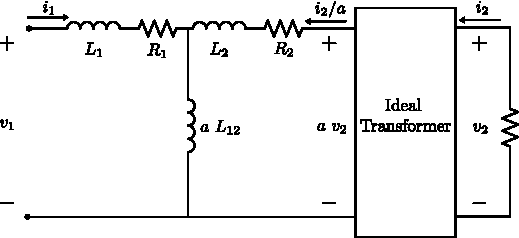
\includegraphics[width=0.8\linewidth]{inkscape_svg/transformer_eq_circuit.pdf}
  \caption{Ideal transformer equivalent circuit.}
  \label{fig:trafo_equivalent}
\end{figure}

% \begin{circuitikz}[american currents, american voltages]

% % Left terminals and v1
% \draw (-1,0) to[open, v=$v_1$] (-1,2);

% % Series elements
% \draw
% (-1,2) to[short, i=$i_1$] (0,2)
%       to[L=$L_1$] (2,2)
%       to[R=$R_1$] (4,2)
%       to[L=$L_2$] (6,2)
%       to[R=$R_2$] (8,2)
%       to[short, i<=$i_2/a$] (9,2);

% % Shunt inductance
% \draw (4,2) to[L=$aL_{12}$] (4,0);

% % Bottom reference
% \draw (-1,0) -- (15,0);

% % Primary-side voltage
% \draw (9,0) to[open, v^=$a\,v_2$] (9,2);

% % Transformer connections
% \draw (9.5,2) -- (12.5,2);
% \draw (9.5,0) -- (12.5,0);

% % Transformer box
% \draw (9.5,0) rectangle (12.5,3);
% \node at (11,1.8) {Ideal};
% \node at (11,1.2) {transformer};
% \node at (11,0.6) {$a\!:\!1$};

% % Secondary side
% \draw
% (12.5,2) to[short, i<=$i_2$] (14.5,2)
%          to[R] (14.5,0);

% % Secondary voltage
% \draw (12.5,0) to[open, v^=$v_2$] (12.5,2);

% \end{circuitikz}

\subsubsection{Numerical model in EMT}

The transformer model is implemented in the EMT simulation using a numerical approach similar to that used for transmission lines using the Dommel method. 
Figure~\ref{fig:dommel_transformer_equivalent} shows the equivalent circuit of the transformer used in the EMT simulation. 

\begin{figure}[H]
  \centering
  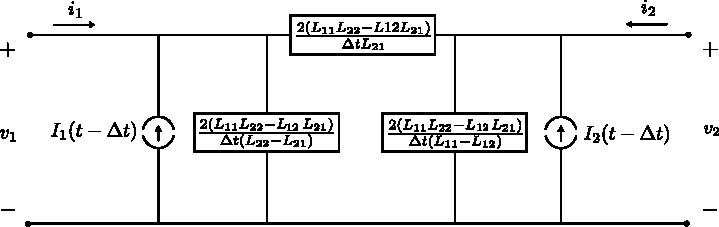
\includegraphics[width=1\linewidth]{inkscape_svg/transformer_dommel.pdf}
  \caption{Ideal transformer equivalent circuit.}
  \label{fig:dommel_transformer_equivalent}
\end{figure}

It's seen how the inductances are represented as a combination of a history component and a conductance derived from the self and mutual inductances. 
From equation~\ref{eq: voltages_transformer}, each winding components are separated as:

\begin{equation}
\frac{d i_1}{d t}
=
\frac{L_{22}}{L_{11}L_{22} - L_{12}L_{21}}\, v_1
-
\frac{L_{21}}{L_{11}L_{22} - L_{12}L_{21}}\, v_2
\end{equation}

\begin{equation}
\frac{d i_2}{d t}
=
-\frac{L_{12}}{L_{11}L_{22} - L_{12}L_{21}}\, v_1
+
\frac{L_{11}}{L_{11}L_{22} - L_{12}L_{21}}\, v_2
\end{equation}

\begin{equation}
L_1 = L_{11} - a L_{12}
\end{equation}
\begin{equation}
L_2 = a^2 L_{22} - a L_{12}
\end{equation}

\begin{equation}
\begin{aligned}
i_1(t)
&= I_{h1}(t-\Delta t)
+ \left(
\frac{L_{22}\,\Delta t}{2\left(L_{11}L_{22}-L_{12}L_{21}\right)}
-
\frac{L_{21}\,\Delta t}{2\left(L_{11}L_{22}-L_{12}L_{21}\right)}
\right) v_1(t) \\
&\phantom{=}
+ \frac{L_{21}\,\Delta t}{2\left(L_{11}L_{22}-L_{12}L_{21}\right)}
\left( v_1(t) - v_2(t) \right)
\end{aligned}
\end{equation}

\begin{equation}
\begin{aligned}
i_2(t)
&= I_{h2}(t-\Delta t)
+ \left(
\frac{L_{11}\,\Delta t}{2\left(L_{11}L_{22}-L_{12}L_{21}\right)}
-
\frac{L_{21}\,\Delta t}{2\left(L_{11}L_{22}-L_{12}L_{21}\right)}
\right) v_1(t) \\
&\phantom{=}
+ \frac{L_{12}\,\Delta t}{2\left(L_{11}L_{22}-L_{12}L_{21}\right)}
\left( v_2(t) - v_1(t) \right)
\end{aligned}
\end{equation}

\begin{equation}
\begin{aligned}
I_{h1}(t-\Delta t)
&= i_1(t-\Delta t)
+ \left(
\frac{L_{22}\,\Delta t}{2\left(L_{11}L_{22}-L_{12}L_{21}\right)}
-
\frac{L_{21}\,\Delta t}{2\left(L_{11}L_{22}-L_{12}L_{21}\right)}
\right) v_1(t-\Delta t) \\
&\phantom{=}
+ \frac{L_{21}\,\Delta t}{2\left(L_{11}L_{22}-L_{12}L_{21}\right)}
\left( v_1(t-\Delta t) - v_2(t-\Delta t) \right)
\end{aligned}
\end{equation}

\begin{equation}
\begin{aligned}
I_{h2}(t-\Delta t)
&= i_2(t-\Delta t)
+ \left(
\frac{L_{11}\,\Delta t}{2\left(L_{11}L_{22}-L_{12}L_{21}\right)}
-
\frac{L_{21}\,\Delta t}{2\left(L_{11}L_{22}-L_{12}L_{21}\right)}
\right) v_1(t-\Delta t) \\
&\phantom{=}
+ \frac{L_{12}\,\Delta t}{2\left(L_{11}L_{22}-L_{12}L_{21}\right)}
\left( v_2(t-\Delta t) - v_1(t-\Delta t) \right)
\end{aligned}
\end{equation}

As seen, formulas for the equivalent current injections can be derived from the equations above and are similar to those used for the lines. 
Some differences between lines and transformers can be highlighted . On the one hand, the currents and history components are calculated with different formulas.
On the other hand, the history component in transformers
delay only in one time-step, while in lines, the delay is $\tau$ depending on the characteristics of each line.

In order to add transformers to the system to be simulated, those are added as lines with different bus voltages at the two ends.

Following the ideal transformer assumption an uncoupled model is assumed for the three-phase transformer. Therefore, the three phases are modelled independently 
without mutual coupling between them and the matrix $G_c$ is diagonal.





